
%(BEGIN_QUESTION)
% Copyright 2011, Tony R. Kuphaldt, released under the Creative Commons Attribution License (v 1.0)
% This means you may do almost anything with this work of mine, so long as you give me proper credit

En DP-transmitter brukes til å måle dampflow gjennom et venturirør:

$$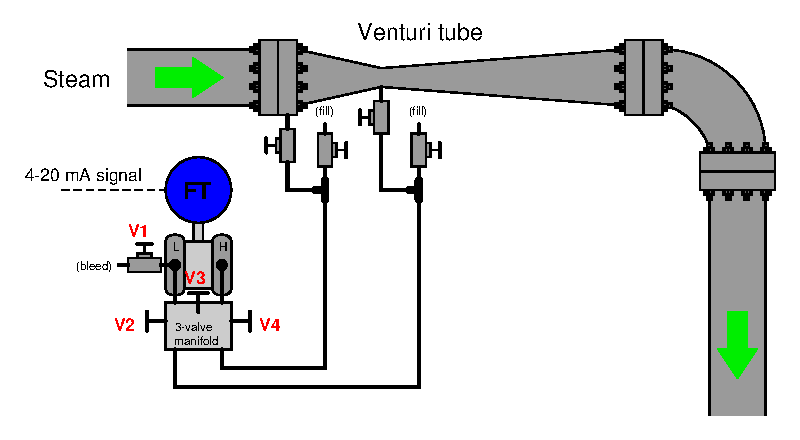
\includegraphics[width=15.5cm]{i01275x01.eps}$$

Angi korrekt stilling for de fire håndventilene som er merket i diagrammet ved normal drift. Kryss enkelt av i riktige ruter i tabellen for å svare på denne delen av spørsmålet:

% No blank lines allowed between lines of an \halign structure!
% I use comments (%) instead, so that TeX doesn't choke.

$$\vbox{\offinterlineskip
\halign{\strut
\vrule \quad\hfil # \ \hfil & 
\vrule \quad\hfil # \ \hfil & 
\vrule \quad\hfil # \ \hfil \vrule \cr
\noalign{\hrule}
%
% First row
Ventil & Åpen & Stengt \cr
%
\noalign{\hrule}
%
% Another row
V1 &   & \cr
%
\noalign{\hrule}
%
% Another row
V2 &   & \cr
%
\noalign{\hrule}
%
% Another row
V3 &   & \cr
%
\noalign{\hrule}
%
% Another row
V4 &   & \cr
%
\noalign{\hrule}
} % End of \halign 
}$$ % End of \vbox

Anta videre at driftspersonell mistenker at denne flowtransmitteren viser feil, og at det er flere år siden transmitteren sist ble kalibrert. Forklar hvordan du kan kontrollere kalibreringen av denne transmitteren, spesielt hvordan du kan avgjøre om feilkalibreringen ligger i {\it sensor trim} (ADC) eller {\it output trim} (DAC), når en HART-kommunikator er ditt {\it eneste} testinstrument. Merk: svaret må forklare hvordan du {\it kontrollerer} om en kalibreringsfeil finnes, ikke hvordan du {\it korrigerer} en kalibreringsfeil, og må spesifikt angi hvilke parametere du vil overvåke med HART-kommunikatoren!

\vskip 50pt

\underbar{file i01275}
%(END_QUESTION)





%(BEGIN_ANSWER)

% No blank lines allowed between lines of an \halign structure!
% I use comments (%) instead, so that TeX doesn't choke.

$$\vbox{\offinterlineskip
\halign{\strut
\vrule \quad\hfil # \ \hfil & 
\vrule \quad\hfil # \ \hfil & 
\vrule \quad\hfil # \ \hfil \vrule \cr
\noalign{\hrule}
%
% First row
Ventil & Åpen & Stengt \cr
%
\noalign{\hrule}
%
% Another row
V1 &  & $\surd$ \cr
%
\noalign{\hrule}
%
% Another row
V2 & $\surd$ &  \cr
%
\noalign{\hrule}
%
% Another row
V3 &  & $\surd$\cr
%
\noalign{\hrule}
%
% Another row
V4 & $\surd$ &  \cr
%
\noalign{\hrule}
} % End of \halign 
}$$ % End of \vbox

\vskip 10pt

Blokker og utlign transmitteren med 3-ventilsmanifolden, og kontroller deretter at kommunikatoren viser null trykkverdi for {\tt PV} -- dette kontrollerer for en sensor trim-feil. Hvis det ikke finnes sensor trim-feil, må den gjenværende kalibreringsfeilen i transmitteren være en output trim-feil.

Merk at kontroll av samsvar mellom vist {\tt PV}-verdi og vist {\tt AO}-verdi i kommunikatoren {\it ikke} kontrollerer verken sensor- eller utgangskalibreringsfeil. Den viste AO-verdien vil stemme med den viste PV-verdien selv om sensor og/eller DAC er grovt feilkalibrert!

\vskip 10pt

Ett poeng for hver ventilstilling, 6 poeng for korrekt forklaring.

%(END_ANSWER)





%(BEGIN_NOTES)

{\bf Dette spørsmålet er ment for eksamener og ikke arbeidsark!}.

%(END_NOTES)

